\documentclass[12pt]{article}                                                                                
\usepackage[utf8]{inputenc}                                                                                  
\usepackage[T1]{fontenc}                                                                                     
\usepackage{amsmath, amssymb}                                                                                
\usepackage{geometry}                                                                                        
\usepackage{xcolor}                                                                                          
\usepackage{lipsum}                                                                                          
\usepackage{titlesec}                                                                                        
\usepackage{fancyhdr}                                                                                        
\usepackage{tcolorbox}                                                                                       
\usepackage{graphicx}                                                                                        
\usepackage{float} % For precise figure placement
\usepackage{tikz}
\usetikzlibrary{arrows.meta, decorations.markings}

\geometry{a4paper, margin=2.5cm}                                                                             
\pagestyle{fancy}                                                                                            
\fancyhf{}                                                                                                   
\rhead{Devoir Maison}                                                                                        
\lhead{Ilyas ZANAN}                                                                                          
\cfoot{\thepage}                                                                                             
                                                                                                             
% Fancy titles                                                                                               
\titleformat{\section}{\normalfont\Large\bfseries}{Exercise \thesection:}{1em}{}                             
\titleformat{\subsection}{\normalfont\bfseries}{Correction:}{1em}{}                                          
                                                                                                             
% Custom box for correction                                                                                  
\tcbuselibrary{listingsutf8}                                                                                 
\newtcolorbox{correctionbox}{                                                                                
  colback=gray!5,                                                                                            
  colframe=black,                                                                                            
  fonttitle=\bfseries,                                                                                       
  title=Correction,                                                                                          
  breakable,                                                                                                 
  before skip=10pt,                                                                                          
  after skip=10pt                                                                                            
}                                                                                                            
                                                                                                             
\begin{document}

% Cover info                                                                                                 
\begin{center}
	\Large\textbf{UNIVERSITY IBN TOFAIL} \\[1em]
	\large\textit{Électorstatique et Magnétostatique} \\[2em]
	\normalsize
	\textbf{Nom:} Ilyas ZANAN \\[0.5em]
	\textbf{Date:} Avril 11, 2025
\end{center}

\vspace{1cm}

% ----------- EXERCISE 1 -------------                                                                       
\section{}
Soient deux charges ponctuelles au repos $q$ et $-q$ placées respectivement en A et en B d'un axe $Ox$. (figure 1)

\begin{figure}[h]
	\centering
	\begin{tikzpicture}[scale=1.2]
		% Line with arrow
		\draw[-latex] (-3,0) -- (3,0) node[right] {$x$};

		% Points
		\fill (0,0) circle (0.05) node[below] {$O$};
		\fill (-1.5,0) circle (0.1) node[below] {$q>0$} node[above] {$A$};
		\fill (1.5,0) circle (0.1) node[below] {$q<0$} node[above] {$B$};

		% Caption
		\node at (-2.5,1.5) {Figure 1};
	\end{tikzpicture}
\end{figure}

\begin{itemize}
	\item Donner l'expression vectorielle de la force électrostatique $\vec{F}_{q/-q}$ créée en B.
	\item Donner l'expression vectorielle du champ électrostatique $\vec{E}$ créé en B.
	\item Donner l'expression du potentiel électrostatique $V$ créé en B.
\end{itemize}

\begin{correctionbox}
	\begin{itemize}
		\item on applique la loi de coloumb on aurra:
		      \begin{displaymath}
			      \begin{align}
				      \vec{F}_{q/-q} = - k_e \frac{q^2}{d^2}\hat{i}
			      \end{align}
		      \end{displaymath}
		\item l'expression vectorielle du champ électrostatique est :
		      \begin{displaymath}
			      \begin{align}
				      \vec{E}_B & = & \frac{\vec{F}_{q/-q}}{-q} \\
				                & = & k_e \frac{q}{d^2}\hat{i}
			      \end{align}
		      \end{displaymath}
		\item l'expression du potentiel électrostatique $V$ créé en B est :
		      \begin{displaymath}
			      \begin{align}
				      V_B & = & k_e \frac{q}{d}
			      \end{align}
		      \end{displaymath}
	\end{itemize}
\end{correctionbox}

\newpage
% ----------- EXERCISE 2 -------------                                                                       
\section{}
Soient deux charges ponctuelles au repos $q$ et $-q$ placées respectivement en A et en B (figure 2).
On donne $OA = OB = a$.

\begin{figure}[h]
	\centering
	\begin{tikzpicture}[scale=1.2]
		% Axes
		\draw[-latex] (-3,0) -- (3,0) node[right] {$x$};
		\draw[-latex] (0,-1) -- (0,3) node[above] {$y$};

		% Unit vectors
		\draw[-latex] (0,0) -- (1,0) node[below] {$\vec{i}$};
		\draw[-latex] (0,0) -- (0,1) node[left] {$\vec{j}$};

		% Points
		\node at (0,0) [below right] {$O$};
		\fill (-1.5,1.5) circle (0.1) node[left] {$q$} node[above] {$A$};
		\fill (1.5,1.5) circle (0.1) node[right] {$-q$} node[above] {$B$};

		% Lines connecting O to A and B
		\draw (0,0) -- (-1.5,1.5);
		\draw (0,0) -- (1.5,1.5);

		% Small 'a' for distance
		\node at (-0.9,0.5) {$a$};
		\node at (0.9,0.5) {$a$};

		% Caption
		\node at (-2.5,-0.5) {Figure 2};
	\end{tikzpicture}
\end{figure}

\begin{itemize}
	\item Donner l'expression vectorielle du champ électrostatique $\vec{E} = E_x \hat{i} + E_y \hat{j}$ créé en O.
	\item Donner l'expression du potentiel électrostatique $V$ créé en O.
\end{itemize}

\begin{correctionbox}
	\begin{itemize}
		\item L'expression vectorielle du champ électrostatique créé en O est :
	\end{itemize}

	\noindent Soit $A(x,y)$ et $B(x',y')$, et $\vec{AO} = \langle -x, -y \rangle$ et $\vec{BO} = \langle -x', -y' \rangle$.

	\begin{align*}
		\vec{E}_A & = k_e \frac{q}{a^2} \frac{\langle -x, -y \rangle}{a}    \\
		          & = k_e \frac{q}{a^3} \langle -x, -y \rangle              \\
		\vec{E}_B & = k_e \frac{-q}{a^2} \frac{\langle -x', -y' \rangle}{a} \\
		          & = k_e \frac{-q}{a^3} \langle -x', -y' \rangle           \\
	\end{align*}

	\noindent Ensuite, on a :
	\begin{align*}
		E_x & = k_e \frac{q}{a^3} (x' - x) \\
		E_y & = k_e \frac{q}{a^3} (y' - y) \\
	\end{align*}
	\noindent Ce qui nous donne :
	\begin{align*}
		\vec{E} & = E_x \hat{i} + E_y \hat{j}                                               \\
		        & = k_e \frac{q}{a^3} (x' - x) \hat{i} + k_e \frac{q}{a^3} (y' - y) \hat{j}
	\end{align*}
\end{correctionbox}

\begin{correctionbox}
	\begin{itemize}
		\item L'expression du potentiel électrostatique créé en O est :
	\end{itemize}

	\begin{align*}
		V_A & = k_e \frac{q}{a}  \\
		V_B & = k_e \frac{-q}{a} \\
	\end{align*}

	\noindent Ce qui nous donne :
	\begin{align*}
		V_{total} & = V_A + V_B                          \\
		          & = k_e \frac{q}{a} -  k_e \frac{q}{a} \\
		          & = 0
	\end{align*}
\end{correctionbox}

\newpage
% ----------- EXERCISE 3 -------------                                                                       
\section{}
Soit un conducteur plan $P_1$ d'épaisseur négligeable et de surface $S$ chargé avec une densité surfacique $\sigma_1 = + \sigma$ perpendiculaire à un axe $XX'$ de vecteur unitaire $\hat{i}$ (\textbf{Voir figure ci-dessous}). Un point $M$ de l'espace est repéré par $\vec{OM}= x \hat{i}$.
\begin{itemize}
	\item Déterminer la charge totale $Q$ de ce conducteur.
	\item Représenter sur le schéma le vecteur champ électrostatique $\vec{E}_1(M)$ crée par ce conducteur en un point M à la distance x du plan pour x>0 et aussi pour x < 0.
\end{itemize}

\begin{figure}[h]
	\centering
	\begin{tikzpicture}[scale=1.2]
		% Axes
		\draw[-latex] (-4,0) -- (4,0) node[right] {$X$};
		\draw (-4,0) node[left] {$X'$};

		% Plate
		\draw[thick] (0,-1) -- (0,1) -- (-1,2) -- (-1,0) -- cycle;
		\node at (-0.5,2.5) {$P_1$};
		\node at (0,0) {$O$};

		% Unit vector
		\draw[dashed, -latex] (0,0) -- (1,0);
		\node at (0.5,0.25) {$\vec{i}$};

		% Caption
		\node at (3,-2) {(Figure 3)};
	\end{tikzpicture}
\end{figure}

\begin{itemize}
	\item En utilisant le théorème de Gauss, Déterminer le champ électrostatique $\vec{E}_1(M)$ crée en un point $M$ à la distance x du plan ($P_1$ est considéré comme infini). Donner les expressions du vecteur champ pout x>0 et pour x<0.
	\item On place parallèlement à $P_1$ à une distance e (figure 4) un autre conducteur plan $P_2$ d'épaisseur négligeable et de surface S chargé avec une densité surfacique $\sigma_2 = - \sigma$. Les deux cnducteurs sont eninfluence total ($P_1$ et $P_2$ sont condidérés comme infinis). \textbf{Déduire le champ électrique $\vec{E}(M)$ crée dans l'espace compris entre ces deux plans }
\end{itemize}

\begin{figure}[h]
	\centering
	\begin{tikzpicture}[scale=1.2]
		% Axes
		\draw[-latex] (-5,0) -- (5,0) node[right] {$X$};
		\draw (-5,0) node[left] {$X'$};

		% First plate
		\draw[thick] (-2,-1) -- (-2,1) -- (-3,2) -- (-3,0) -- cycle;
		\node at (-2.5,2.5) {$P_1$};
		\node at (-2,0) {$O$};

		% Second plate
		\draw[thick] (2,-1) -- (2,1) -- (1,2) -- (1,0) -- cycle;
		\node at (1.5,2.5) {$P_2$};

		% Unit vector
		\draw[dashed, -latex] (-2,0) -- (-1,0);
		\node at (-1.5,0.25) {$\vec{i}$};

		% Distance
		\draw[<->] (-2,-1.5) -- (2,-1.5);
		\node at (0,-1.25) {$e$};

		% Caption
		\node at (4,-2) {(Figure 4)};
	\end{tikzpicture}
\end{figure}

\begin{itemize}
	\item soient $V_1$ et $V_2$ respectivement les potentiels électrostatiques de $P_1$ et $P_2$. \\ \textbf{Determiner la capacité de ce condensateur dans le cas où (S>>e)}.
	\item En utilisant l'expression de la densité d'énergie $\frac{d \omega}{dV} = \frac{\epsilon_0}{2}E^2$, \\ \textbf{Déterminer l'énergie électrostatique emmagasinée dans ce condensateur en fonction de $Q$, $V_1$ et $V_2$}.
\end{itemize}

\begin{correctionbox}
	\begin{itemize}
		\item La charge total est $Q = \sigma \times S$
	\end{itemize}

	\begin{itemize}
		\item
	\end{itemize}
	\centering
	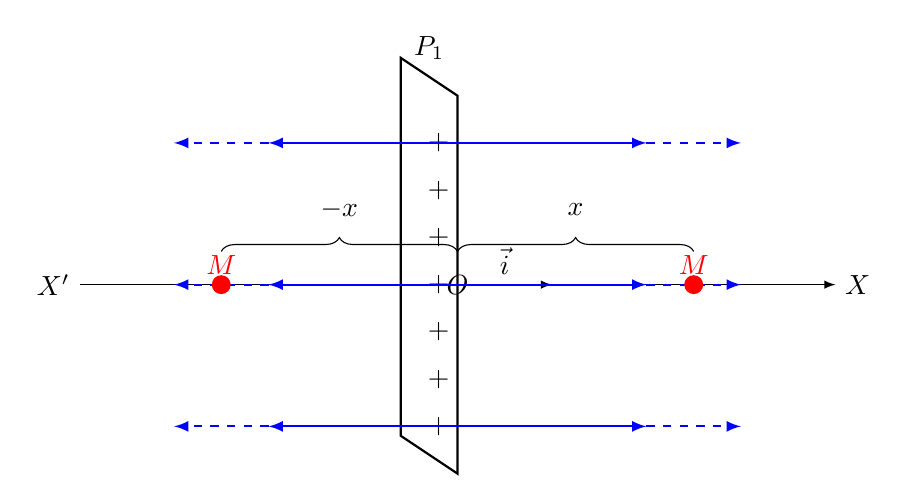
\begin{tikzpicture}[scale=1.2]
		% Axes
		\draw[-latex] (-4,0) -- (4,0) node[right] {$X$};
		\draw (-4,0) node[left] {$X'$};

		% Plate (like in Figure 3, but smaller)
		\draw[thick] (0,-2) -- (0,2) -- (-0.6,2.4) -- (-0.6,-1.6) -- cycle;
		\node at (-0.3,2.5) {$P_1$};
		\node at (0,0) {$O$};

		% Positive charges (adjusted for new plate)
		\foreach \y in {-1.5,-1,-0.5,0,0.5,1,1.5}
			{
				\node at (-0.2,\y) {$+$};
			}

		% Unit vector (reversed direction)
		\draw[dashed, -latex] (0,0) -- (1,0);
		\node at (0.5,0.25) {$\vec{i}$};

		% Electric field vectors (right side)
		\foreach \y in {-1.5,0,1.5}
			{
				\draw[-latex, blue, thick] (0,\y) -- (2,\y);
				\draw[-latex, blue, thick, dashed] (2,\y) -- (3,\y);
			}

		% Electric field vectors (left side)
		\foreach \y in {-1.5,0,1.5}
			{
				\draw[-latex, blue, thick] (0,\y) -- (-2,\y);
				\draw[-latex, blue, thick, dashed] (-2,\y) -- (-3,\y);
			}

		% Points with distance labels
		\fill[red] (2.5,0) circle (0.1) node[above] {$M$};
		\fill[red] (-2.5,0) circle (0.1) node[above] {$M$};

		% Distance labels
		\draw [decorate, decoration={brace, amplitude=5pt}, yshift=10pt] (0,0) -- (2.5,0)
		node [black, midway, yshift=15pt] {$x$};
		\draw [decorate, decoration={brace, amplitude=5pt}, yshift=10pt] (-2.5,0) -- (0,0)
		node [black, midway, yshift=15pt] {$-x$};

	\end{tikzpicture}
	\begin{itemize}
		\item D'apres le theorem de Gauss On a :
	\end{itemize}
	\begin{align*}
		     & \vec{E}_1 (M)  = \frac{\sigma_1}{2\epsilon_0} \hat{\eta} \\
		\iff & \vec{E}_1 (M)  =
		\begin{cases}
			\frac{\sigma}{2\epsilon_0} \hat{i},   & x >0 \\
			- \frac{\sigma}{2\epsilon_0} \hat{i}, & x <0 \\
		\end{cases}
	\end{align*}

	\begin{itemize}
		\item On a :
	\end{itemize}
	\begin{align*}
		\vec{E}_1 = \frac{\sigma}{2\epsilon_0} \hat{i} \\
		\vec{E}_2 = \frac{\sigma}{2\epsilon_0} \hat{i} \\
	\end{align*}
	\noindent $\vec{E}_2$ est positive care on a $P_1$ est derrière $P_2$, Avec $\sigma_2 = - \sigma$:
	\begin{align*}
		\vec{E}_2 & = - \frac{\sigma_2}{2\epsilon_0} \hat{i} \\
		          & = \frac{\sigma}{2\epsilon_0}
	\end{align*}

\end{correctionbox}

\begin{correctionbox}
	\noindent D'où:
	\begin{align*}
		\vec{E}_T & = \vec{E}_1 + \vec{E}_2             \\
		          & = \frac{\sigma}{\epsilon_0} \hat{i}
	\end{align*}
	\begin{itemize}
		\item On a d'aprés la derrière question : $\vec{E} =\frac{\sigma}{\epsilon_0} \hat{i}  $, d'ou :
	\end{itemize}
	\begin{align*}
		V             & = E \times e                  \\
		              & = \frac{\sigma}{\epsilon_0} e \\
		              & = \frac{Qe}{\epsilon_0 S}     \\
		\Rightarrow C & = \frac{Q}{V}                 \\
		              & = \frac{\epsilon_0 S}{e}
	\end{align*}
	\noindent Lorsque la surface $S$ des plaques est beaucoup plus grande que leur séparation $e$ ($S>>e$), cela donne un champ électrique uniforme entre les plaques.

	\begin{itemize}
		\item On utilisons la relation $\frac{d \omega}{dV} = \frac{\epsilon_0}{2}E^2$, On a:
	\end{itemize}

	\noindent La densité d'énergie :
	\begin{align*}
		\frac{d\omega}{dV} & = \frac{\epsilon_0}{2} E^2                                        \\
		                   & = \frac{\epsilon_0}{2} \left( \frac{\sigma}{\epsilon_0} \right)^2 \\
		                   & = \frac{\epsilon_0}{2} \cdot \frac{\sigma^2}{\epsilon_0^2}        \\
		                   & = \frac{\sigma^2}{2\epsilon_0}.
	\end{align*}

	\noindent L'énergie total:
	\begin{align*}
		U & = \int \frac{d\omega}{dV} \, dV                  \\
		  & = \int \frac{\sigma^2}{2\epsilon_0} \, dV        \\
		  & = \frac{\sigma^2}{2\epsilon_0} \cdot V           \\
		  & = \frac{\sigma^2}{2\epsilon_0} \cdot (S \cdot e) \\
		  & = \frac{\sigma^2 S e}{2\epsilon_0}.
	\end{align*}
\end{correctionbox}

\begin{correctionbox}
	\noindent L'énergie total en fonction de $Q,V_1$ et $V_2$:
	\begin{align*}
		U & = \frac{\sigma^2 S e}{2\epsilon_0}                                                                                                   \\
		  & = \frac{\left( \frac{Q}{S} \right)^2 S e}{2\epsilon_0} \quad \text{(car $ \sigma = \frac{Q}{S} $)}                                   \\
		  & = \frac{\frac{Q^2}{S^2} S e}{2\epsilon_0}                                                                                            \\
		  & = \frac{Q^2 e}{2\epsilon_0 S}                                                                                                        \\
		  & = \frac{Q^2}{2\epsilon_0 S} \cdot \frac{V \epsilon_0 S}{Q} \quad \text{(car $ e = \frac{V \epsilon_0 S}{Q} $, où $ V = V_1 - V_2 $)} \\
		  & = \frac{Q^2 V}{2 Q}                                                                                                                  \\
		  & = \frac{1}{2} Q V                                                                                                                    \\
		  & = \frac{1}{2} Q (V_1 - V_2).
	\end{align*}
\end{correctionbox}

\end{document}
